% LTeX: language=en-GB
% !TeX root = ..\Thesis.tex
\section{The final product}\label{sec:07}
This section will demonstrate the resulting workflow of the project for some various setups.
\subsection{Running the device}
The simplest workflow is running a DUT for some number of cycles. Consider \cref{lst:runDut}.
\begin{listing}
    \centering
    \caption{Running an ALU for 40 cycles}\label{lst:runDut}
    \begin{minted}{java}
        SteelBrew steelBrew = new SteelBrew();
        steelBrew.clean();
        Forge.enableWSL(true);
        Brewer alu = new Brewer("alu");
        alu.clocks(40);
        alu.runDUT();
        Forge.simulate();
    \end{minted}
\end{listing}
Line 1 initialises SteelBrew and the Forge. Hereafter the root folder is cleaned for leftover files from previous simulations. Line 3 enables the Windows Subsystem for Linux support. On line 4 the ALU is added as the DUT. Line 5 sets the number of running cycles to 40 and 6 creates a testbench that simply runs the DUT for 40 cycles. On line 7 the program begins the simulation. The resulting file \texttt{waveformalurun.vcd} can then be inspected. The resulting screenshot is shown on \cref{fig:runDut}.
\begin{figure}
    \centering
    \caption{Waveform after running the ALU for 40 cycles}\label{fig:runDut}
    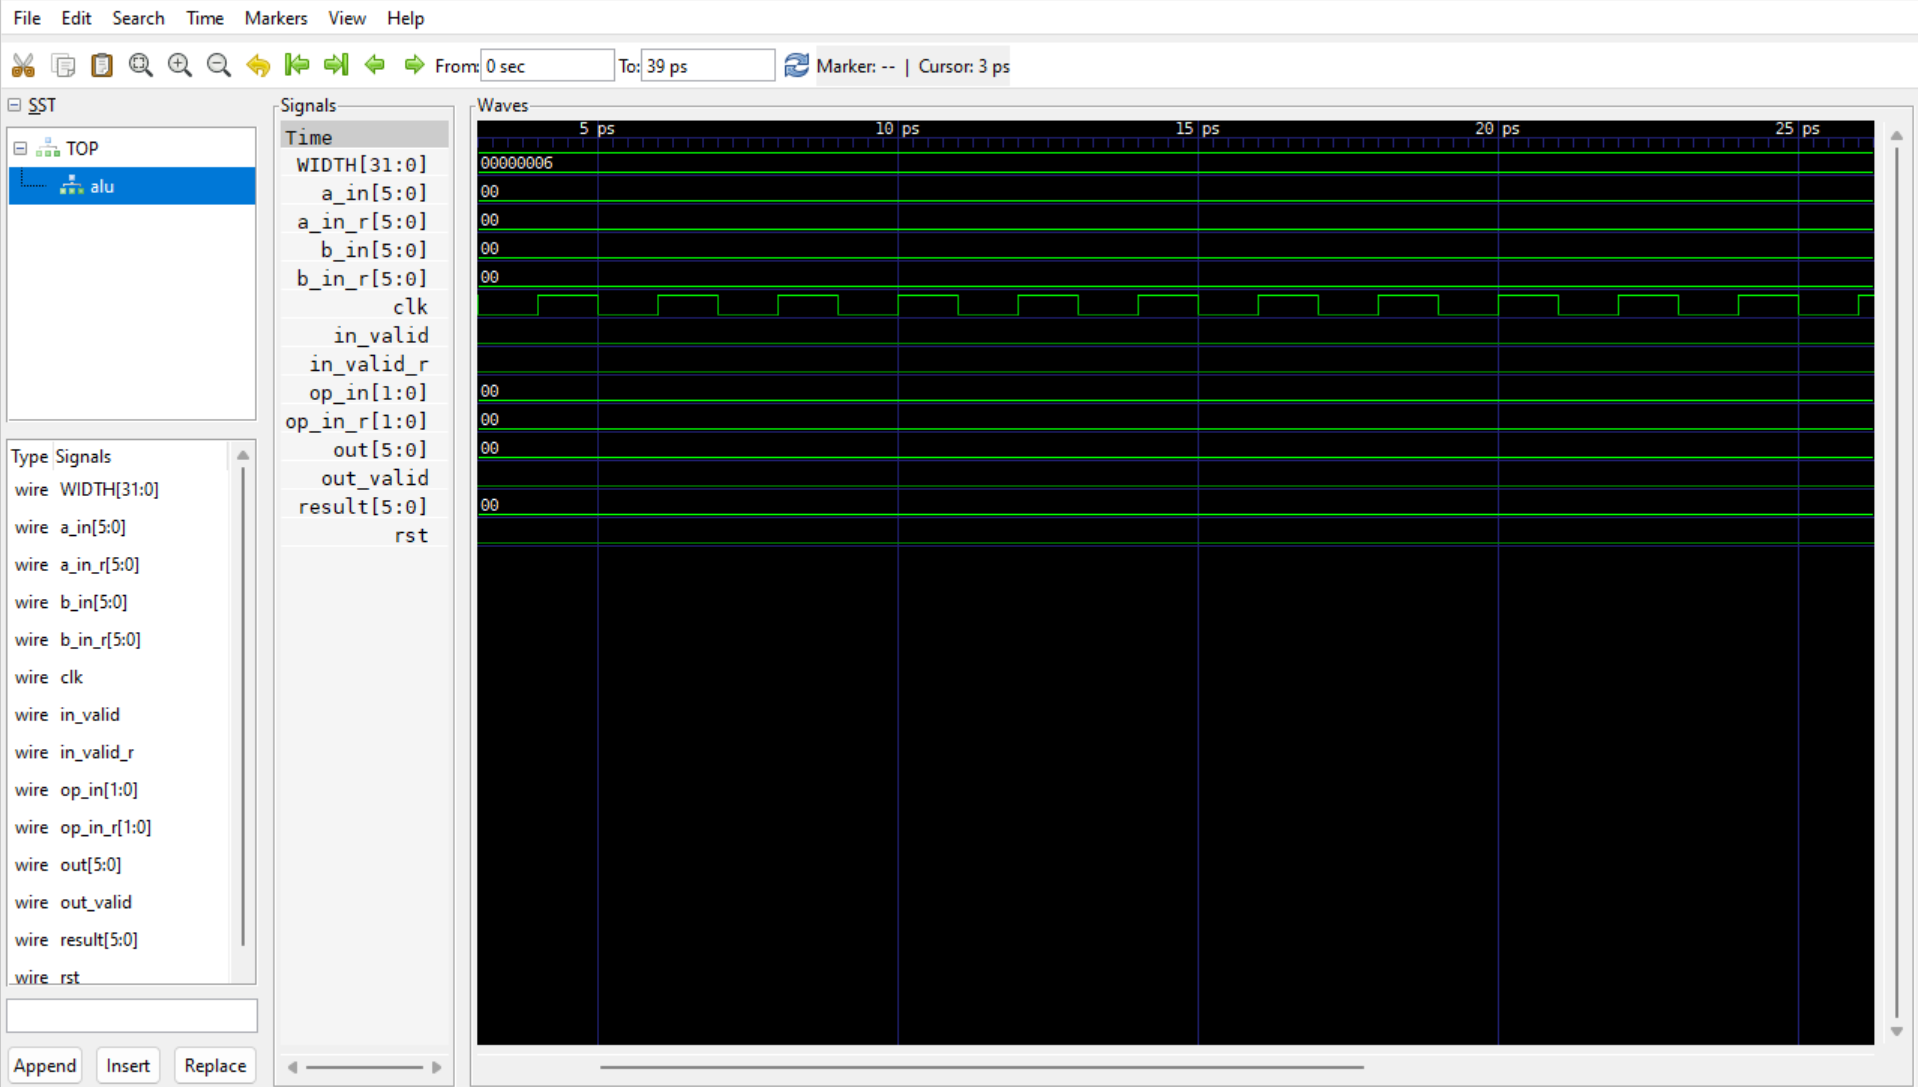
\includegraphics[width=.8\textwidth]{graphics/runDUT.png}
\end{figure}
As seen from the figure, the ALU ran from 0 to 39 ps and the \texttt{clk} signal is behaving as expected. The simplest case works.
\subsection{Peek, poke and step}
For the next workflow, the listing is shown on \cref{lst:peekpokestep}.
\begin{listing}
    \centering
    \caption{Peek, poke, and step used on an ALU}\label{lst:peekpokestep}
    \begin{minted}{java}
        SteelBrew steelBrew = new SteelBrew();
        steelBrew.clean();
        Forge.enableWSL(true);
        Brewer alu = new Brewer("alu");
        Batch batch = new Batch("PeekPokeStep");
        Signal signal = new Signal("in_valid", 1);
        batch.addSignal(signal);
        batch.peek(signal);
        batch.poke(signal, BigInteger.ONE);
        batch.step();
        batch.peek(signal);
        batch.step();
        batch.poke(signal, BigInteger.ZERO);
        batch.step();
        batch.peek(signal);
        batch.step();
        batch.step();
        alu.brew(batch);
        Forge.simulate();
    \end{minted}
\end{listing}
Lines 1-5 is seen in the previous example. On line 6 the variable \texttt{signal} is pointed to ``\texttt{in\_valid}'', and on line 7 the signal is added to the batch. Lines 8–15 peeks at the signal, changes it to 1, peeks and changes it to 0, with some clock steps in-between. 16-17 starts the simulation. \cref{fig:peekpokestep} shows the resulting console output and \cref{fig:peekpokestepWave} shows the signal.
\begin{figure}
    \centering
    \caption{Console output after using peek, poke and step on the ALU}\label{fig:peekpokestep}
    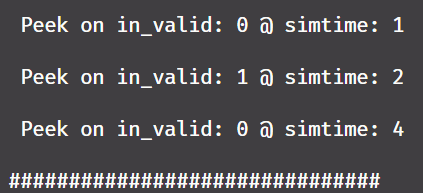
\includegraphics[width=.3\textwidth]{graphics/peekpokestep.png}
\end{figure}
\begin{figure}
    \centering
    \caption{Waveform changes with and poke}\label{fig:peekpokestepWave}
    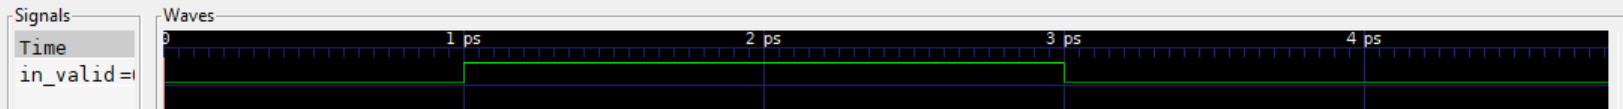
\includegraphics[width=\textwidth]{graphics/peekpokestepWave.png}
\end{figure}
The wave and the console output behaves as expected.
\subsection{Expect}
This next workflow demonstrate how to look for expected values. Consider \cref{lst:expect}.
\begin{listing}
    \centering
    \caption{Expecting signal in the ALU}\label{lst:expect}
    \begin{minted}{java}
        SteelBrew steelBrew = new SteelBrew();
        steelBrew.clean();
        Forge.enableWSL(true);
        Brewer alu = new Brewer("alu");
        Batch batch = new Batch("Expect");
        Signal signal = new Signal("in_valid", 1);
        batch.addSignal(signal);
        batch.step();
        batch.expect(signal, BigInteger.ONE);
        batch.peek(signal);
        batch.step();
        alu.brew(batch);
        Forge.simulate();
    \end{minted}
\end{listing}
The new addition here is line 9. We expect the signal to be a 1. \cref{fig:expectConsole} shows the console output.
\begin{figure}
    \centering
    \caption{Console output after using expect on the ALU}\label{fig:expectConsole}
    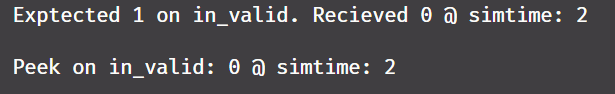
\includegraphics[width=.5\textwidth]{graphics/expectConsole.png}
\end{figure}
Exactly as expected.
\subsection{Assertions}
Regrettably, the assertion methods did not work as expected. After rigorous experimentation, it would seem like the approach employed in the Assert method is inherently flawed. Placing the while loop in the testbench is needed for the current assertion-logic, however it rules out the possibility for peek and poke during a batch containing assertions. Further investigation is needed. Perhaps some randomised initial conditions combined with the expect method, would stand in for assertions, but this is truly not the way either.
\subsection{Concurrency}
When executing multiple batches, the forge successfully runs multiple threads as seen on \cref{fig:concurr}.
\begin{figure}
    \centering
    \caption{Multiple instances of Verilator created by Barista}\label{fig:concurr}
    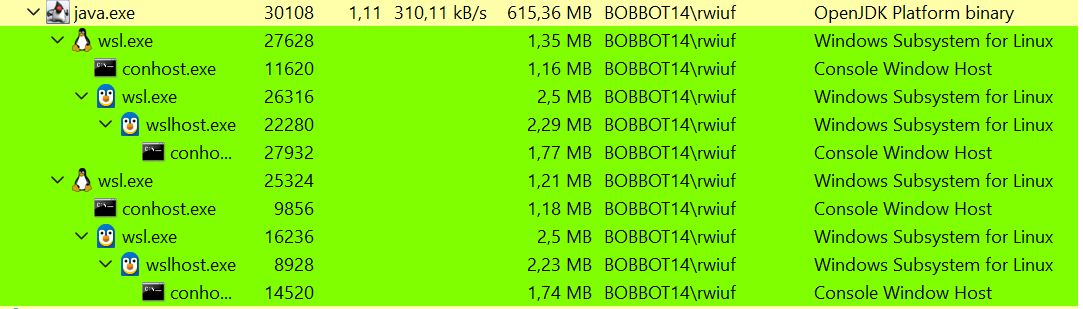
\includegraphics[width=.8\textwidth]{graphics/concurrency.png}
\end{figure}
This combined with Verilator's lightweight approach, and possibly, by employing its multithreading capabilities could dramatically speed up the verification process.
\subsection{Further development}
The groundwork is laid for further development. The development tasks would be as follows:
\begin{enumerate}
    \item Implement working Assertions.
    \item Employ Verilator multithreading.
    \item Expand assertions with assume and cover logic.
\end{enumerate}
The project as-is would be easily extendable with other testing capabilities, and as it is written in Java, the user could use their own logic, to prepare and execute tests.